\documentclass[../m134a-hw2.tex]{subfiles}

\begin{document}

\subsection*{5}
At any given time, prove that there are two points on the surface of the earth diametrically opposite
from each other that have the exact same temperature.

Since two diametrically opposed points on a sphere lie on a single plane, we can take a slice of the spherical earth through the center to produce a circle with the two diametrically opposed points.

We will parametrize the temperature on the ring as $T(\theta)$ where we pick any point on the circle and assign its $\theta$ to zero. 
Then, $\theta$ represents a another point on the circle by the angle created from that point, the center of the ring, and the chosen $\theta_0$.

So, given that the period of a circle is $2\pi$, then $T(\theta)=T(\theta+2\pi)$.

We can assume that this function will be continuous because, between any two points with different temperatures, there must exist a point in between with a temperature in between as well.

\begin{figure*}[ht] %h: place figure about here
\centering
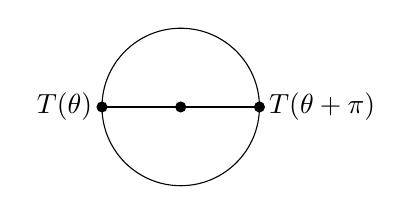
\begin{tikzpicture}
    \draw (0,0) circle (1);

    \draw (-1,0) -- (1,0);

    \node at (-1,0) [left] {$T(\theta)$};
    \node at (1,0) [right] {$T(\theta+\pi)$};

    \fill (0,0) circle[radius=2pt];
    \fill (-1,0) circle[radius=2pt];
    \fill (1,0) circle[radius=2pt];
\end{tikzpicture}
\end{figure*}

The two diametrically opposed points are $T(\theta)$ and $T(\theta+\pi)$.

We seek some $\theta$ such that the difference between between these two points is zero.

So, we will let $f$ represent the different between the temperature at one point and its opposing point on the other hemisphere, \[f(\theta) = T(\theta) - T(\theta+\pi).\]
The difference of the continuous function $T(\theta)$ with a horizontal offset of itself $T(\theta + a)$ is also continuous. Therefore $f$ is continuous.

We will show that there exists a $c$ such that $f(c) = 0$.

First, we note that going measuring the temperature in one direction is the same as measuring temperature in the opposite direction. 
\begin{align*}
    f(\theta + \pi) &= T(\theta + \pi) - T(\theta + 2\pi) \\
    f(\theta + \pi) &= T(\theta + \pi) - T(\theta) \\
    f(\theta + \pi) &= -\left(T(\theta) - T(\theta + \pi)\right) \\
    f(\theta + \pi) &= -f(\theta) \\
\end{align*}

If $f(\theta) = 0$, then $f(\theta + \pi) = 0$.

This is analogous to a constant temperature at all points. So, for all pairs of points by $a$, $f(a) = 0$.
In this case, the statement holds.

So, we can now assume $|f(\theta)| > 0$ which implies $|f(\theta + \pi)| > 0$.

Since $f(\theta)$ and $f(\theta + \pi)$ have the opposite signs, there must exist a $K = 0$ in between because $f$ is continuous.

So, there exists a $c \in [0,\pi]$ such that $f(c) = K = 0$ by the IVT.

Therefore, since we need to trace over one half of the circle, $[0,\pi]$ to check for equal points on the other half, $[\pi,2\pi]$, the statement is true.

\subsection*{6}
A hiker begins a backpacking trip at 6am on Saturday morning, arriving at camp at 6pm that evening. 
The next day, the hiker returns on the same trail leaving at 6am in the morning and finishing at 6pm. 
Show that there is some place on the trail that the hiker visited at the same time of day both coming and going.

Let the interval $[0,2a] = [0,a] \cup [a,2a]$ define the total duration of the journey where $a$ is the twelve-hour one-way duration.

Assume that the journey ranges from a minimum starting position 0 to some maximum position $x_0 > 0$.

We will represent the first first trip by $f(t)$ and the second by $g(t)$.
We assume that these functions are continuous because the hiker cannot teleport and therefore must pass through all intermediary positions between any two given positions.

It is given that the starting point of $f$ by the same as the ending point of $g$ where both are the starting position 0, $f(0)=0=g(2a)$.

Then, it is also given that the ending point of $f$ is th same as the starting point of $g$, which is the maximum $x_0$, $f(a)=x_0=g(a)$

We can then visualize the two functions $f$ and $g$,

\begin{figure*}[ht]
\centering
\begin{tikzpicture}
    % axes
    \draw[->] (0,0) -- (6,0) node[right] {$t$};
    \draw[->] (0,0) -- (0,4) node[above] {$x$};

    \node[left] (x_0) at (0,3) {$x_0$};
    \node[left] (0x) at (0,0) {$0$};
    % ticks
    \draw[thick] (-0.1,0) -- (0.1,0);
    \draw[thick] (-0.1,3) -- (0.1,3);

    \node[below] (0t) at (0,0) {$0$};
    \node[below] (a) at (2.5,0) {$a$};
    \node[below] (2a) at (5,0) {$2a$};    
    % ticks
    \draw[thick] (0,-0.1) -- (0,0.1);
    \draw[thick] (2.5,-0.1) -- (2.5,0.1);
    \draw[thick] (5,-0.1) -- (5,0.1);

    \draw[dashed] (x_0) -- (2.5,3);

    % mock paths
    \draw[blue] (0,0) .. controls (2,1) and (0,3) .. (2.5,3);
    \draw[red] (2.5,3) .. controls (3,3) and (4,0) .. (5,0);

    \node[left] at (1,2) {\textcolor{blue}{$f$}};
    \node[right] at (3.5,2) {\textcolor{red}{$g$}};
\end{tikzpicture}
\end{figure*}

\begin{comment}
THE INTERMEDIATE-VALUE THEOREM
If f is continuous on [a, b] and K is any number between f (a) and f (b), then
there is at least one number c in the interval (a, b) such that f (c) = K.
\end{comment}

We can also expand the domain of $f$ to include $[a,2a]$ where its value remains constant at $x_0$.
We can do the same for $g$ such that its value is the minimum 0 on $[0,a]$. Therefore, both functions are defined and continuous on the total interval $[0,2a]$.

Then, we define $h(t) = f(t) - g(t + a)$ which represents the difference in position between $f$ and $g$ after their starting time. Since both $f$ and $g$ are continuous on $[0,2a]$, their difference is also continuous.

When $h$ is zero, the hiker's position $f$ and $g$ will be the same at the same time in the journey.

So, we seek a $c$ such that $h(c) = 0$.

For $t = 0$, we have, $h(0) = f(0) - g(a) = 0 - x_0 =-x_0$.

For $t = a$, we have, $h(a) = f(a) - g(2a) = x_0 - 0 = x_0$.

Since $x_0 > 0$, then $-x_0 < 0 x_0$.

So, there exists a $c \in [0,a]$ such that $h(c) = 0$ by the IVT.

Therefore, there is some point $c$ that the hiker will visit at the same time after starting the journey on each day.

\end{document}